%--------------------------------------------------
%  Topología – Clase 5
%--------------------------------------------------
\subsection{Topología producto.}

\paragraph{\textbf{Definición. (Topologia producto)}} 
Las siguientes definiciones son equivalentes:
\begin{enumerate}[label=(\roman*)]
  \item Dados $X$ y $Y$ espacios topológicos, la topología producto en $X \times Y$  es la minima topología que hace a las proyecciones:
  \begin{align*}
    \pi_1: X \times Y \to X
  \end{align*}
  \begin{align*}
    \pi_2: X \times Y \to Y
  \end{align*}  
  continuas.

  \item Es la topología generada por la subbase:
  \begin{align*}
    \{
   \pi_1^{-1}(U) : U  \overset{\text{ab}}\subseteq X \} \cup \{
      \pi_2^{-1}(V) : V  \overset{\text{ab}}\subseteq Y \}
  \end{align*}
  \item Es la topología generada por la base:
  \begin{align*}
    \mathcal B = \{ U \times V : U \subseteq^{ab } X, V \subseteq^{ab } Y \}
  \end{align*}
\end{enumerate}

\paragraph{Nota} Un disco es abierto, pero no es resultado de producto cartesiano de abiertos.


\paragraph{\textbf{Proposición.}} $\mathbb R^n - \{0\}  \simeq  S^{n-1} \times \mathbb R$,.

% es decir la n-1 esfera prodcuto cruz $\mathbb R$.
\paragraph{\textbf{Demostración.}}

Se toma la esfera unitaria en $\mathbb R^n$  alrededor del origen, luego tomamos un $\mathbf v$ y luego consideramos su proyección a la esfera. Asi definimos 

\shorthandoff{<>}
\begin{figure}[H]
  \centering
  %--------------------------------------------------
  %  Deformación continua:  \R^n\setminus\{0\}  ->  S^{n-1}\times\R
  %--------------------------------------------------
  %
  %  Fase 1 (0–10):     círculo   ->   cono
  %  Fase 2 (11–20):    cono      ->   cilindro
  %
  \begin{animateinline}[poster=first,controls,loop]{10}%
    \multiframe{21}{iFrame=0+1}{%
      % Parámetro normalizado t in [0,1]
      \pgfmathsetmacro{\t}{\iFrame/20}%
      %---------- Primer tramo (0 <= t <= 0.5) : círculo -> cono ----------
      \pgfmathsetmacro{\tA}{min(2*\t,1)}            % 0→1 en la primera mitad
      \pgfmathsetmacro{\rCircle}{1.5*(1-\tA)}       % radio del círculo
      \pgfmathsetmacro{\hCone}{3*\tA}               % altura del cono
      %---------- Segundo tramo (0.5 < t <= 1) : cono -> cilindro ----------
      \pgfmathsetmacro{\tB}{max(2*(\t-0.5),0)}      % 0→1 en la segunda mitad
      \pgfmathsetmacro{\hCylLow}{-1.5}              % fondo del cilindro
      %
      \begin{tikzpicture}[scale=1]
        % Eje de referencia solo al principio (opcional)
        \ifdim \t pt<0.02pt
          \draw[-, black, thick] (0,-2) -- (0,-.1);
          \draw[->, black, thick] (0,.1) -- (0,2) node[above] {$y$};

          \draw[-, black, thick] (-2,0) -- (-.1,0);
          \draw[->, black, thick] (.1,0) -- (2.,0) node[right] {$x$};

          %Draw circule in center
          \draw[blue, thick] (0,0) circle (.1);
        \fi
        % ----------  círculo / esfera  ----------
        \ifdim \rCircle pt>0pt
        \draw[-, black, thick] (0,-2) -- (0,-.1);
        \draw[->, black, thick] (0,.1) -- (0,2) node[above] {$y$};

        \draw[-, black, thick] (-2,0) -- (-.1,0);
        \draw[->, black, thick] (.1,0) -- (2.,0) node[right] {$x$};

        %Draw circule in center
        \draw[blue, thick] (0,0) circle (.1);
          \draw[purple, thick] (0,0) circle (\rCircle);
        \fi
        % ----------  cono  ----------
        \ifdim \hCone pt>0pt
          \ifdim \tB pt<0.02pt
            \draw[purple, thick] (-.1,0) -- ({-1.2*\tA},{\hCone});
            \draw[purple, thick] (.1,0) -- ({ 1.2*\tA},{\hCone});
            \draw[blue, dotted] ({-.1},{0}) arc (180:0:{.1} and {0.1});
            \draw[blue]        ({-.1},{0}) arc (180:360:{.1} and {0.1});
            % borde superior del cono
            \draw[purple, dashed] ({-1.2*\tA},{\hCone}) arc (180:0:{1.2*\tA} and {0.3*\tA});
            \draw[purple]        ({-1.2*\tA},{\hCone}) arc (180:360:{1.2*\tA} and {0.3*\tA});
          \fi
        \fi
        \ifdim \tB pt>0pt
          % radio inferior: 0.1  →  1  (crece linealmente con t_B)
          \pgfmathsetmacro{\rBot}{0.1 + 0.85*\tB}
          % aristas laterales: del borde superior (radio 1) al borde inferior (radio \rBot)
          \draw[purple, thick] (-1,2) -- ({-\rBot},\hCylLow);
          \draw[purple, thick] ( 1,2) -- ({ \rBot},\hCylLow);
              % elipse superior (radio fijo = 1)
          \draw[purple, dashed] (-1,2) arc (180:0:1 and 0.3);
          \draw[purple]        (-1,2) arc (180:360:1 and 0.3);

              % elipse inferior (radio variable = \rBot)
          \draw[blue, dashed] ({-\rBot},\hCylLow) arc (180:0:{\rBot} and 0.3);
          \draw[blue]        ({-\rBot},\hCylLow) arc (180:360:{\rBot} and 0.3) node[right] {$S^1$};
          % círculo central (S^1) – simple indicador
          
        \fi
        % ----------  cilindro  ----------
        % \ifdim \tB pt>0pt
        %   \draw[purple, thick] (-1,2) -- (-1,\hCylLow);
        %   \draw[purple, thick] ( 1,2) -- ( 1,\hCylLow);
        %   \draw[purple, dashed] (-1,2) arc (180:0:1 and 0.3);
        %   \draw[purple]        (-1,2) arc (180:360:1 and 0.3);
        %   \draw[purple, dashed] (-1,\hCylLow) arc (180:0:1 and 0.3);
        %   \draw[purple]        (-1,\hCylLow) arc (180:360:1 and 0.3);
        %   % círculo central (S^1)
        %   \draw[blue, thick] (0,0.2) ellipse (0.7 and 0.3);
        %   \node at (0.9,0.2) {$S^1$};
        % \fi
      \end{tikzpicture}%
    }% end multiframe
  \end{animateinline}
  \shorthandon{<>}
  \caption{Deformación continua que visualiza el homeomorfismo $\mathbb{R}^n \setminus \{0\} \simeq S^{n-1}\times\mathbb{R}$.}
\end{figure}
\begin{align*}
\phi : \mathbb R^n - \{0\} &\to S^{n-1} \times \mathbb R^{+} \sim S^{n-1} \times \mathbb R\\
\mathbf v &\mapsto \left( \frac{\mathbf v}{||\mathbf v||}, ||\mathbf v|| \right)
\end{align*}
y $\phi$ es continua desde el calculo vectorial.
Ahora definamos:
\begin{align*}
\psi: S^{n-1} \times \mathbb R &\to \mathbb R^n - \{0\}\\
(\mathbf w, \lambda) &\mapsto \lambda \cdot \mathbf w
\end{align*}
y considerando la composición:
\begin{align*}
(\psi \circ \phi)(\mathbf v) &= \psi \left( \frac{\mathbf v}{||\mathbf v||}, ||\mathbf v|| \right)=\mathbf v
\end{align*}
Ahora sea 
\begin{align*}
(\phi \circ \psi)(\mathbf w, \lambda) &= \phi(\lambda \cdot \mathbf w) = \left( \frac{\lambda \cdot \mathbf w}{||\lambda \cdot \mathbf w||}, ||\lambda \cdot \mathbf w|| \right)\\
&= \left( \frac{\lambda \cdot \mathbf w}{|\lambda| \cdot ||\mathbf w||}, |\lambda| \cdot ||\mathbf w|| \right)\\
&= \left(\mathbf w, \lambda\right) \qquad \text{Notemos que }  S^{n-1} = \{ \mathbf v \in \mathbb R^n : ||\mathbf v|| = 1 \} \text{ por eso $||w||=1$}
\end{align*}

Luego $\phi$  es un homomeomorfismo. Ademas
\begin{align*}
\zeta: \mathbb R^+ &\to \mathbb R \quad \text{es un homeomorfismo} \\
x& \mapsto \ln(x)\\
\end{align*}
\begin{align*}
\zeta^{-1}: \mathbb R &\to \mathbb R^+ \quad \text{es un homeomorfismo} \\
x& \mapsto e^x\\ 
\end{align*}

Luego $\mathbb R^+ \simeq \mathbb R$. 

También definimos
\begin{align*}
(id, \zeta) \circ \phi : S^{n-1} \times \mathbb R^+ &\to S^{n-1} \times \mathbb R\\
(\mathbf w, \lambda) &\mapsto (\mathbf w, \ln(\lambda))\\
\end{align*}

define un homomeomorfismo entre $\mathbb R^{n} - \{0\}$ y $S^{n-1} \times \mathbb R$. De este modo:

\begin{align*}
  \mathbb R^n - \{0\} &\simeq S^{n-1} \times \mathbb R^{+} \simeq S^{n-1} \times \mathbb R\\
\end{align*}

\paragraph{Ejercicio.} Demostrar que $\zeta$ y $\zeta^{-1}$ son continuas.
\paragraph{Ejercicio.} Ahora $S^{1} \times[a,b]$ es homeomorfo  a una corona 

\paragraph{\textbf{Proposición.}} Una función $f: Z \to X \times Y$ es continua si y solo si 
\begin{align*}
\Pi_1 \circ f: Z &\to X
\end{align*}
\begin{align*}
\Pi_2 \circ f: Z &\to Y\\
\end{align*}

Son continuas.

\paragraph{\textbf{Demostración.}} 
\begin{itemize}
  \item [$\implies$] OEMS ($\Pi_1$, $\Pi_2$ y $f$ son continuas, y la composición de funciones continuas es continua).
  \item [$\impliedby$]  (Ejercicio observacion)
  Si $\mathcal B$ es una subbase de $Y$ y $f:X\to Y$ es continua sii $f^{-1}(B) \overset{\text{ab}}\subseteq X$, para todo $B \in \mathcal B$.
  
  Sea $\Pi_1^{-1}(U)$ un abierto de la subbase de la top producto ($U\overset{\text{ab}}\subseteq X$), queremos ver que:
  \begin{align*}
  f^{-1}(\Pi_1^{-1}(U)) \overset{\text{ab}}\subseteq Z
  \end{align*}
 donde: 
 \begin{align*}
  \Pi_1 \circ f: Z &\to X\\
  \Pi_2 \circ f: Z &\to Y\\
 \end{align*}
 Ahora $f^{-1}(\Pi_1^{-1}(U)) =  (\Pi_1 \circ f)^{-1}(U) \overset{\text{ab}}\subseteq Z$ pues $\Pi_1 \circ f$ es continua. Análogamente se muestra que:
 $f^{-1}(\Pi_2^{-1}(V)) \overset{\text{ab}}\subseteq Z$ para todo $V \overset{\text{ab}}\subseteq Y$
\end{itemize}


\paragraph{\textbf{Ejercicios}}

\begin{itemize}
  \item Hatcher cap 1:
  \begin{itemize}
    \item 12
    \item 15
  \end{itemize}
  \item Viro, Ivanov:
  \begin{itemize}
    \item 20E
    \item 20.24
    \item 20.31
    \item 20.R
    \item $[20'8]$
    \item 20.Y
  \end{itemize}
\end{itemize}

Fin del primer capitulo.

\subsection{Conexidad.}
Existen propiedades que nos permitas diferenciar espacios, e identificar propiedades. que hacen a un espacio mas tratable. La conexidad es una de esta propiedades. Intuitivamente un espacio es conexo si tiene solo una parte, si un hombrecito se para en un punto, puede recorrer todo el espacio
\begin{center}
  \begin{animateinline}[poster=first,controls,loop]{12}% FPS = 12
    \multiframe{41}{i=0+1}{%
      % --------- Parámetro normalizado t = i/40  -------------
      \pgfmathsetmacro{\t}{\i/40}%
      % --------- Parametrización cúbica de la curva -----------
      \pgfmathsetmacro{\x}{ 2.4*\t*\t - 1.4*\t*\t*\t }%
      \pgfmathsetmacro{\y}{ 0.95*\t*\t*\t
                            -2.25*\t*\t
                            +2.25*\t
                            +0.05 }%
      % --------- Dibujo --------------------------------------
      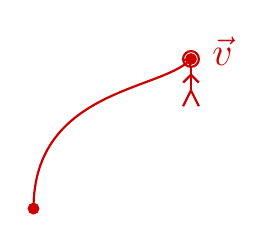
\begin{tikzpicture}[scale=2,
                          every node/.style={font=\small}]
        % Trayectoria de referencia
        \draw[red!80!black,thick,->]
              (0,0.05) .. controls (0,0.8) and (0.8,0.8) .. (1,1);
        % Puntos inicial y final
        \draw[fill=white,thick,red!80!black] (0,0.05) circle (0.03);
        \draw[fill=white,thick,red!80!black] (1,1)    circle (0.03);
        % Vector v
        \node[red!80!black,font=\Large] at (1.2,1.05) {$\vec{v}$};
        % Hombrecito desplazado a (x(t),y(t))
        \begin{scope}[shift={(\x,\y)},red!80!black,thick]
          \draw (0,0) circle (0.05);          % cabeza
          \draw (0,-0.05) -- (0,-0.2);        % torso
          \draw (0,-0.1) -- (-0.05,-0.15);    % brazo izq.
          \draw (0,-0.1) -- ( 0.05,-0.15);    % brazo der.
          \draw (0,-0.2) -- (-0.05,-0.3);     % pierna izq.
          \draw (0,-0.2) -- ( 0.05,-0.3);     % pierna der.
        \end{scope}
      \end{tikzpicture}
    }% end multiframe
  \end{animateinline}
  
\end{center}

\paragraph{\textbf{Ejemplos (Conexos).}}
\begin{itemize}
  \item $\mathbb R^n$ es conexo.
  \item $\mathbb R^n - \{0\}$ con la topología de subespacio si $n \geq 2$.
\end{itemize}

\paragraph{\textbf{No conexos.}}
\begin{itemize}
  \item $\{a,b\}$ en la topología discreta.
  \item $(a,b) \cup (c,d)$ subespacio de \(\mathbb R\) 
  \item $\mathbb R^n - \{0\}$ cuando $n=1$, con la topología de subespacio.
\end{itemize}

\subsubsection{Formalización.}


\paragraph{\textbf{Definición.}} $X$ es conexo si no es posible descomponerlo como la union de dos abiertos no vacíos disyuntos, lo cual significa que si
\begin{align*}
X = A \cup B \quad \text{con } A,B \overset{\text{ab}}\subseteq X, A,B \neq \emptyset \quad \implies  \quad A \cap B \neq \emptyset
\end{align*}
\paragraph{\textbf{Ejemplo.}}
\begin{enumerate}[label=(\alph*)]
  \item $X = (a,b) \cup (c,d)$, $b<c$ no es conexo porque $(a,b)\overset{\text{ab}}\subseteq X$ y $(c,d)\overset{\text{ab}}\subseteq X$, y $(a,b)\cap(c,d)=\emptyset$. Es un espacio disconexo.
  \item $(X,\mathcal T_{\mathrm{discreta}})$ con $|X|>1$: sea $a\in X$, entonces
        \[
          X = \{a\} \sqcup (X \setminus \{a\}), 
        \]
        con ambos en la topología discreta, por lo que $X$ es disconexo.
\end{enumerate}

El espacio-tiempo es conexo, que ocurre alrededor de eso con el tunelamiento cuántico?

\paragraph{\textbf{Teorema}} $[a,b]$ es conexo.

\paragraph{\textbf{Demostración.}}: Consideremos lo siguientes casos:

\begin{enumerate}[label=(\Roman*)]
  \item $\emptyset$ es vacíamente conexo.
  \item $a=b \implies [a,b] = \{a\}$ es conexo. Un singleton es siempre conexo.
  \item $a<b$. Supongamos que $[a,b] = A \sqcup B$, con $A,B \overset{\text{ab}}\subseteq [a,b]$, entonces $A,B \overset{\text{cerr}}\subseteq [a,b]$, pues por definición de la topología de subespacio (Clase 3) ($[a,b]/A,[a,b]/B \in \mathcal T_{[a,b]}$, significa $A,B$ son cerrados en $[a,b]$). Supongamos que $a\in A$, entonces existe un $\epsilon > 0$ tal que $[a,a+\epsilon) \overset{\text{ab}}\subseteq A$, Luego existe $c \in [a, a+\epsilon)$ tal que $c>a$ y $[a,c] \subseteq A$. Por lo que definimos:
  
  \begin{center}
    \shorthandoff{<>}
    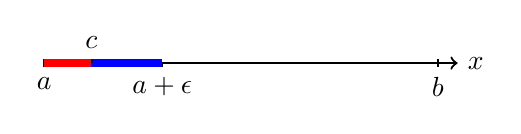
\begin{tikzpicture}[x=5cm, y=1cm]  % Escala horizontal ampliada
      % Dibuja la recta [a,b]
      \draw[thick,->] (0,0) -- (1.05,0) node[right] {\(x\)};
      \foreach \pos/\label in {0/a,1/b} {
        \draw[thick] (\pos,0.05) -- (\pos,-0.05) node[below] {\(\label\)};
      }

      % Definiciones numéricas de ejemplo
      \pgfmathsetmacro{\eps}{0.3}      % epsilon en escala [0,1]
      \pgfmathsetmacro{\cpos}{0.4*\eps} % posición de c = a + 0.4*epsilon

      % Marca a+epsilon y resalta [a, a+epsilon]
      \coordinate (ae) at (\eps,0);
      \draw[thick] (ae) -- ++(0,-0.05) node[below] {\(a+\epsilon\)};
      \draw[line width=3pt,blue] (0,0) -- (ae);

      % Marca c y resalta [a, c]
      \coordinate (c) at (\cpos,0);
      \draw[thick] (c) -- ++(0,0.05) node[above] {\(c\)};
      \draw[line width=3pt,red] (0,0) -- (c);
    \end{tikzpicture}
    \shorthandon{<>}
  \end{center}
  
  \begin{align*}
  C= \{c\in \mathbb R: [a,c] \subseteq A\}
  \end{align*}
  Veamos Si $b\in C$, $A = [a,b]$ y $B = \emptyset$. (una forma alternativa es $X =A \cup B$, $A,B \overset{\text{ab}}\subseteq$ $A\neq \emptyset \implies B =\emptyset$ ). Para esto veamos que:
  \begin{itemize}
    \item $C \neq \emptyset$ por que $a\in C$.
    \item $C$ es acotado superiormente, por que $b$ es una cota superior de $C$. Si $[a,c] \subseteq A\subseteq [a,b]$, esto es $c\leq b$. Por lo que $C$ tiene  supremo. Asi queremos ver que $\sup C = b$:
    \begin{itemize}
      \item  $\sup C >a$. Existe $c>a$ tal que $c \in C$, por lo que $a$ no es cota superior de $C$.
      \item $\sup C \in C$, $[a,\sup C] \subseteq A$. Queremos ver que el $\sup C$ es un punto limite de $A$. Sea $U$ vecindad básica del $\sup C$ en $[a,b]$. Tenemos que ocurre uno de los siguientes:
      \begin{itemize}
        \item $U = (\sup C - \epsilon, \sup C + \epsilon)$.
        \item $U = (\sup C - \epsilon, \sup C]$
      \end{itemize}
      En cualquier caso $(\sup C - \epsilon, \sup C] \subseteq U$. Queremos ver que $U \cap A \neq \emptyset$. Notemos $\sup C - \epsilon/2$ no es cota superior de $C$, existe $c \in C$ tq $c\geq \sup C - \epsilon/2$, luego $[a,c] \subseteq A$,entonces $c \in A$. Entonces existe $c \in U \cap A \neq \emptyset$. Luego $\sup C$ es un punto limite de $A$.
      \item Como $A$ es cerrado, $A$ contiene todos sus puntos limites, por lo que $\sup C \in A$.
    \end{itemize}
    \item Sea $c \in [a,\sup C] \subseteq A$, $\sup C \in C$. Consideremos:
    
    \begin{align*}
    \bigcup_{c \in C} [a,c] = [a,\sup C) \subseteq A
    \end{align*}
    
    
    \item Pero como el $\sup C \in A$ entonces $[a,\sup C] \subseteq A$. Es decir $\sup C \in C$. 
    \item Supongamos que $\sup C < b$, y $[a, \sup C] \subseteq A$, pero $A$ es abierto entonces $\epsilon > 0$ tal que $[a, \sup C + \epsilon) \subseteq A$, y $[a,\sup C] \subseteq [a,\sup C + \epsilon)$, luego  $\sup C + \epsilon/2 \in C$ luego esto no es posible por la propiedad del supremo.  Entonces $\sup C = b$. Es decir $[a,b] \subseteq A$, y entonces $B = \emptyset$, luego $[a,b]$ es conexo.
    
  \end{itemize}

\end{enumerate}


\paragraph{\textbf{Observación.}}: Conexidad se preserva  por homeomorfismos.

\paragraph{\textbf{Teorema}}: Sea $A \subseteq X$ si $A\subseteq B \subseteq \overline A$, si $A$ es conexo, entonces $B$ es conexo.

\paragraph{\textbf{Demostración.}}: Supongamos que $B$ Se desompone en $B = C \cup D$, donde $C,D$ son abiertos disjuntos no vacios. Intersectando con $A$

$A = (C \cap A) \cup (D \cap A)$, donde $C \cap A$ y $D \cap A$ son abiertos disjuntos de $A$, Entonces o bien $A\subseteq A$ o $A\subseteq D$. Por ejemplo si $A \subseteq C$ entonces $\overline A \subseteq \overline C$, Continuara JAJAJAJ.
